\documentclass[a4paper]{book}
%\documentclass[a4paper]{ctexbook}
%\documentclass[a4paper]{ctexart}
\usepackage{ctex}
\usepackage{listings}
\usepackage{xcolor}
\usepackage{graphicx}
\usepackage{hyperref} %生成书签

%================================
% A.PDF标签
%================================
\hypersetup{
    colorlinks=true,
    bookmarksnumbered=true,
    pdftitle={My LaTeX2e note},
    pdfkeywords={LaTex, note},
}

\title{\Huge \bfseries 使用 \LaTeX 编写笔记}
\author{\huge 莫志烨}
\CTEXoptions[today=big]
\date{\Large \today}

%================================
% B.代码全局格式
%================================
\lstset{
    numbers=left,
    %numberstyle={\color{lightgray}},
    numberstyle={\color{green}},
    backgroundcolor={\color[RGB]{41, 47, 51}}, %背景颜色
    basicstyle={\color[RGB]{208, 214, 219}}, %普通字符串颜色
    stringstyle={\color[RGB]{0, 128, 0}}, %字符串颜色
    keywordstyle={\color[RGB]{101, 140, 230}}, %关键词颜色
    commentstyle={\color{gray}}, %注释颜色
    frame=none, %无边框
    breaklines=true, %自动分行
    language={[ANSI]C},
    captionpos=b,
}

%================================
% C.新命令定义
%================================
%\newcommand{OutputListing}[]{
%}

\begin{document}

%================================
% 1.标题
%================================
\chapter{标题}
\begin{titlepage}
\maketitle
\end{titlepage}

%================================
% 2.目录
%================================
\chapter{目录}
\tableofcontents

%================================
% 3.章节(每天日志入口)
%================================
\chapter{LaTex笔记}
\section{每天日志格式}

%1.每天日志格式

1.每天日志格式
\begin{lstlisting}[]
\chapter{2020年3月3日} //1.以日期为章节
\section{问题1} //2.以问题为小节!
\end{lstlisting}

2.插入代码格式1
\begin{lstlisting}[]
\begin{lstlistings}[caption={xxx}] %插入图注 //默认是C语法
\end{lstlistings}
\end{lstlisting}

2.插入代码格式2
\begin{lstlisting}[]
\lstinputlisting{lbuf.c}[caption={xxx}] %插入图注!
\end{lstlisting}

2.插入代码格式3
\begin{lstlisting}[]
\lstinline !code!
\end{lstlisting}

3.插入图片格式
\begin{lstlisting}[]
\graphicspath{{note_everyday/001_20200302/picture/}} %声明图片加载路径
\begin{figure}[h] %h:表示把图片放在当前位置
    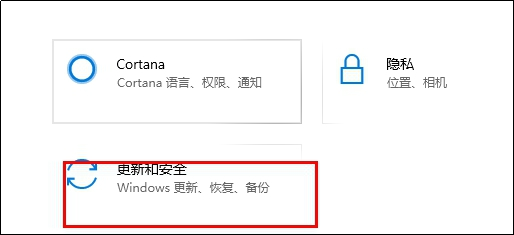
\includegraphics{001.jpg}
    \caption{第一步}
\end{figure}

\end{lstlisting}

\chapter{2020年3月2日 笔记}
\graphicspath{{note_everyday/001_20200302/picture/}}
\section{问题一:MMU学习}


1.步骤一:
\begin{figure}[h]
    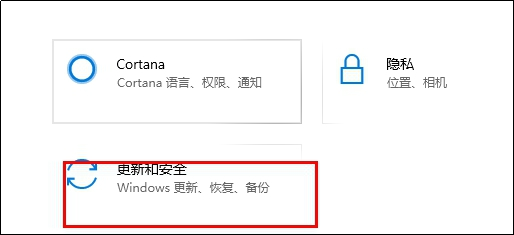
\includegraphics{001.jpg}
    \caption{第一步}
\end{figure}



\chapter{2020年3月5日 笔记}
\graphicspath{{note_everyday/004_20200305/picture/}}
\section{IIC协议}

1.接线 \\
    1)SCL: 时钟线, 由主机提供;\\
    2)SDA: 数据线;\\
    idle状态两个信号都会被拉高;\\

2.总线状态\\
    1)空闲状态: SCL和SDA都保持着高电平;\\
    2)start信号: 当SCL为高电平而SDA由高到低的跳变,表示产生一个起始条件;\\
    3)stop信号: 当SCL为高而SDA由低到高的跳变,表示产生一个停止条件;\\
    4)传输状态(忙): 处于start <---> stop之间;\\
        传输状态数据格式:数据采用: 8bit数据(发送方) + 1(接收方ack把SDA拉低);\\
        注: 整个过程取决于谁在控制SDA, 数据由发送方控制SDA状态发送, ack由接收方控制拉低(此时接收方为输入检测状态); \\

3.主机流程分析\\

4.主机流程分析\\


问题Q1:
1) 作为主机, 在发完数据后需要发stop信号时, 因为需要关enable, 但由于波特率太慢问题, 指令执行的太快, 在IIC模块还没发出stop信号, cpu就把模块关了;
\begin{lstlisting}[]
    if (end) {
    	iic_host_send_stop(iic_regs[id]); //stop singal
		//asm ("csync");
		delay(100);
		iic_disable(iic_regs[id]);
    }
\end{lstlisting}
    A.软件初步解决办法: 加delay();
    B.IC解决办法: 加stop pending, 等stop pending起来后再disable;

问题Q2: 作为主机, 在发完stop信号后, 再start, 信号会变得不正常(看stp看出时cnt问题);

\begin{figure}[h]
    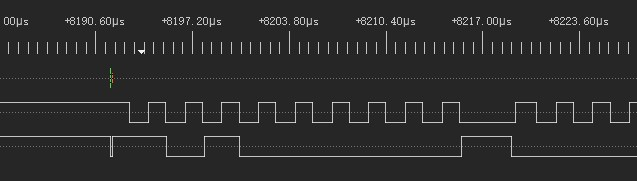
\includegraphics{q2_singal.jpg}
    \caption{第一步}
\end{figure}

问题Q3: 在读时不支持: 在不stop的情况下start
\begin{figure}[h]
    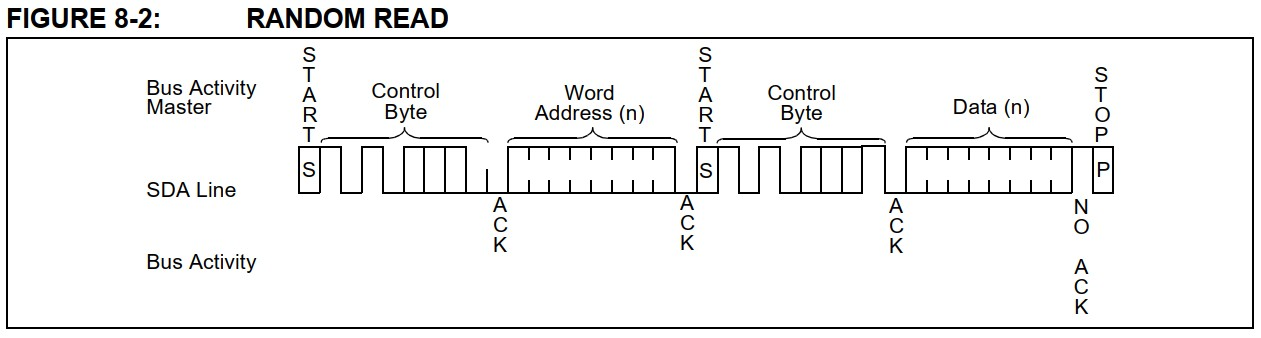
\includegraphics{eeprom_random_read.jpg}
    \caption{第一步}
\end{figure}




\chapter{2020年3月6日 笔记}
\graphicspath{{note_everyday/005_20200306/picture/}}
\section{VOA}

%Big companies are trying to keep their employees healthy by banning business trips. The decision, however, has been a hard blow to the travel industry, which has already been suffering because of the effects of the new coronavirus.
大型企业正试图通过禁止商务旅行来确保员工的健康。但是这一决定给已经因为新型冠状病毒遭受重创的旅游业造成了沉重打击。
Amazon, the American-based online business, has told its nearly 800,000 workers to postpone any unnecessary travel within the United States or around the world.
总部位于美国的网络公司亚马逊已经通知其近80万员工推迟在美国国内或全球范围内任何非必要的旅行。

Swiss food company Nestle told its 291,000 employees worldwide to limit local business travel and stop all international travel until March 15.
瑞士食品公司雀巢通知该公司在全球的29.1万名员工,在3月1日前要限制当地商务旅行并停止所有全球旅行。

France's L'Oréal, maker of beauty products, employs 86,000 people. It has announced a travel ban until March 31.
法国美容产品制造商欧莱雅公司雇用了8.6万名员工。该公司宣布3月31日前禁止旅行。

Major business gatherings, like the Mobile World Congress in Barcelona, have also been canceled.
诸如巴塞罗那世界移动大会之类的大型商业聚会也都被取消。

On Tuesday, Facebook confirmed it will not attend the South by Southwest conference in Austin, Texas. The event is supposed to start on March 13.
周二,脸书网确认将不会参加在德克萨斯州奥斯汀市举行的西南偏南大会。该活动原定于3月13日开幕。

In addition, the International Monetary Fund and the World Bank have announced they will replace their spring meetings in Washington with an online event.
此外,国际货币基金组织和世界银行宣布将通过线上活动替代他们在华盛顿的春季会议。

Robin Ottaway is president of Brooklyn Brewery. He canceled a trip to Seoul and Tokyo last week. He has suspended all travel to Asia and canceled a planned trip this month to Copenhagen.
罗槟·奥特韦是布鲁克林啤酒厂的总裁。他上周取消了前往首尔和东京的旅行。他已经暂停前往亚洲,并取消了本月原计划前往哥本哈根的旅行。

"I wasn't worried about getting sick. I'm a healthy 46-year-old man," Ottaway said. "My only worry was getting stuck in Asia or quarantined after returning to the U.S. And I'd hate to be a spreader of the virus."
奥特韦表示:“我不是害怕感染。我是一位46岁的健康男性。我唯一担心是被困在亚洲,或是回到美国后被隔离。我不想成为这种病毒的传播者。”

Effect on business travel
对商务旅行的影响

The cancellations and travel restrictions are hurting the travel industry. Business travel makes up around 26 percent of the total travel spending, or around $1.5 trillion per year, notes the Global Business Travel Association.
取消和旅行限制伤害了旅游业。全球商务旅行协会指出,商务旅行约占整个旅行支出的26%,即每年大约1.5万亿美元。

The association estimates the virus is costing the business travel industry $47 billion per month.
该协会估计该病毒每个月给商务旅行行业造成470亿美元的损失。

"It's a big deal," said Henry Harteveldt, a travel industry expert. He estimates that airline companies get 55 percent of their money from business travelers because they often sit in pricier business or first-class seats.
旅游行业专家亨特·哈特威尔特表示:“这是个大事件。”他估计航空公司55%对收入来自于商务旅客,因为他们通常乘坐价格更高的商务舱或头等舱。

Numbers from the Airlines Reporting Corporation show that airline ticket sales fell about 9 percent in late February, compared with a year earlier.
航空报告公司的数据显示,与去年同期相比,2月下旬的机票销售下降了大约9%。

Hotel operators are also worried about decreases in business travel. In the United States, hotels are expected to earn $46 billion from business travel this year, said the travel research service Phocuswright. No one believes that is possible now.
酒店经营者也在担心商务旅行的减少。旅游研究公司Phocuswright表示,美国酒店今年预计从商务旅行中赚到460亿美元。现在没人相信这能实现。

In the week through February 22, hotel occupancy rates in San Francisco were down 11 percent, noted STR, a company that researches hotel usage. Several major companies pulled out of the city's cybersecurity conference, which began in February.
研究酒店入住率的STR公司指出,截至2月22日的这个星期,旧金山酒店入住率下降了11%。几家重要公司退出了该市2月份开始举行的网络安全会议。

Some observers say it is wise for companies to postpone or cancel travel before things get worse. Worldwide, the coronavirus has sickened over 90,000 people. More than 3,000 have died from COVID-19, the disease resulting from the virus.
一些观察人士表示,企业在情况恶化前取消或推迟旅行是非常明智的。在全球范围内,这种冠状病毒已经导致9万人感染。超过3千人因为这种病毒引起的新型冠状病毒肺炎死亡。

Kevin Mitchell is chairman of the Business Travel Coalition. He is an expert in the ways large companies and governments can control travel costs. He notes that if a company puts an employee at risk, "you can be held responsible for their injury or death."
凯文·米切尔是商务旅行联盟的主席。他是大型企业和政府差旅成本控制方面的专家。他指出,如果企业将员工置于危险之中,“可能需要对他们的伤亡负责。”
By Susan Shand
05 March 2020
Big companies are trying to keep their employees healthy by banning business trips. The decision, however, has been a hard blow to the travel industry, which has already been suffering because of the effects of the new coronavirus.

Amazon, the American-based online business, has told its nearly 800,000 workers to postpone any unnecessary travel within the United States or around the world.

Swiss food company Nestle told its 291,000 employees worldwide to limit local business travel and stop all international travel until March 15.

Workers wearing protective gear spray disinfectant as a precaution against the coronavirus outbreak, in the departure terminal at the Rafik Hariri International Airport, in Beirut, Lebanon, Thursday, March 5, 2020.
France's L'Oréal, maker of beauty products, employs 86,000 people. It has announced a travel ban until March 31.

Major business gatherings, like the Mobile World Congress in Barcelona, have also been canceled.

On Tuesday, Facebook confirmed it will not attend the South by Southwest conference in Austin, Texas. The event is supposed to start on March 13.

In addition, the International Monetary Fund and the World Bank have announced they will replace their spring meetings in Washington with an online event.

Robin Ottaway is president of Brooklyn Brewery. He canceled a trip to Seoul and Tokyo last week. He has suspended all travel to Asia and canceled a planned trip this month to Copenhagen.

"I wasn't worried about getting sick. I'm a healthy 46-year-old man," Ottaway said. "My only worry was getting stuck in Asia or quarantined after returning to the U.S. And I'd hate to be a spreader of the virus."

Effect on business travel

The cancellations and travel restrictions are hurting the travel industry. Business travel makes up around 26 percent of the total travel spending, or around 1.5 trillion per year, notes the Global Business Travel Association.

The association estimates the virus is costing the business travel industry 47 billion per month.

"It's a big deal," said Henry Harteveldt, a travel industry expert. He estimates that airline companies get 55 percent of their money from business travelers because they often sit in pricier business or first-class seats.

Numbers from the Airlines Reporting Corporation show that airline ticket sales fell about 9 percent in late February, compared with a year earlier.

Hotel operators are also worried about decreases in business travel. In the United States, hotels are expected to earn 46 billion from business travel this year, said the travel research service Phocuswright. No one believes that is possible now.

In the week through February 22, hotel occupancy rates in San Francisco were down 11 percent, noted STR, a company that researches hotel usage. Several major companies pulled out of the city's cybersecurity conference, which began in February.

Some observers say it is wise for companies to postpone or cancel travel before things get worse. Worldwide, the coronavirus has sickened over 90,000 people. More than 3,000 have died from COVID-19, the disease resulting from the virus.

Kevin Mitchell is chairman of the Business Travel Coalition. He is an expert in the ways large companies and governments can control travel costs. He notes that if a company puts an employee at risk, "you can be held responsible for their injury or death."

I'm Susan Shand.

The Associated Press reported this story. Susan Shand adapted it for VOA Learning English. George Grow was the editor.

Write to us in the Comments Section or on 51VOA.COM.

%________________________________________________________________

Words in This Story
outbreak – n. a sudden start or increase of fighting or disease

cosmetics – n. a substance (such as a cream, lotion, or powder) that you put on your face or body to improve your appearanc

standstill – n. a state in which all activity or motion is stopped

quarantine – v. to keep (a person or animal) away from others to prevent a disease from spreading

cybersecurity – n. ways to keep internet data away from criminals


\chapter{2020年3月16日 笔记}
\graphicspath{{note_everyday/001_20200316/picture/}}
\section{VOA}
%\begin{document}
\begin{lstlisting}[]
By Susan Shand
15 March 2020
Billionaire art collector David Nahmad cannot remember why he bought "Nature Morte," a small oil painting by Pablo Picasso.
Nahmad owns about 300 of Picasso's works. So, his forgetfulness is understandable.
"We bought so many Picassos now, I don't remember the... reason," Nahmad said to Associated Press reporters from his home in Monaco.
The 72-year-old started dealing art with his brothers in the 1960s, paying as little as 5,000 for pieces by Picasso and building the collection of works that made them into billionaires.
"Nature Morte" is the smallest painting Nahmad has. And it is about to belong to someone else. It will be sold to raise money for charity later this month.
Raffle tickets will be sold online and are 100 euros each. The winner of a similar Picasso raffle in 2013 was a 23-year-old worker from Pennsylvania.
Nahmad is one of the art world's most important art dealers. He will receive over 1 million for "Nature Morte." But he said the piece is worth "at least two, three times" that.
"This raffle would not have succeeded if the name was not Picasso. I tried to propose other artists' names. But it would not work, because they wanted a name that would appeal to everybody. It has to be Picasso. Picasso is the magic name," he said.
The value of Nahmad's collection is estimated to be about 3 billion. But he himself will not say what the exact value is.
"I don't think people care about the number of works, but about their quality," he said.
Nahmad said the possibility of giving up "Nature Morte" has made him look more closely at the small still life painting. It shows a newspaper and a glass of alcohol on a wood table.
"I think this painting is extremely chic," Nahmad said.
The raffle will be held in Paris on March 30. The organizers hope to sell 200,000 tickets. The money the event raises will help provide water for villagers in Cameroon, Madagascar and Morocco.
Nahmad believes that Picasso, who died in 1973, would have liked the raffling of his works to the public.
"Picasso was very generous," Nahmad said. "He wanted his art to be collected by all kinds of people, not only by the super-rich."
Nahmad's hope is that the winner of "Nature Morte" will be someone who loves the work. If not, "I will be very unhappy" and "would like to buy it back," Nahmad said.
"There's nothing worse than to own something without understanding that thing," he said.
I'm Susan Shand.
The Associated Press reported this story. Susan Shand adapted it for VOA Learning English. Ashley Thompson was the editor.
Write to us in the Comments Section or on 51VOA.COM.

\newline
%________________________________________________________________

Words in This Story
charity - n. the act of giving money, food, or other kinds of help to people who are poo

raffle – n. a contest that a group or organization uses to earn money and that involves people buying numbered tickets in exchange for a chance to win a prize

propose – v. to suggest (something, such as a plan or theory) to a person or group of people to consider

magic - n. special power, influence, or skill

chic – adj. following the current fashion or style : fashionable and appealing

generous - adj. freely giving or sharing money and other valuable things

%\end{document}
\end{lstlisting}







\end{document}



%This is 日志.

